\documentclass[11pt, xcolor={dvipsnames}, hyperref={colorlinks, allcolors=Blue}]{beamer}


% Packages
\usepackage{graphicx}
\usepackage{caption, subcaption}
\usepackage{tikz}
\usepackage{amsmath, amsfonts, amssymb}
\usepackage{bm}
\usepackage{booktabs}
\usepackage{apacite}
\usepackage{multirow}
\usepackage{multicol}
\usepackage{doi}
\usepackage{textpos}
\usepackage{lipsum}
\usepackage{amsfonts, amsmath}
\usepackage{wrapfig}
\usepackage{animate}
\usepackage{cleveref}


\renewcommand\doiprefix{}


\usepackage{tikz}
\usetikzlibrary{shapes, fit}





%%%%%%%%%%%%%%%%%%%%%%%%%%%%%%%%%%%%%%%%%%%%%%
% Custom commands
\newcommand\bc[1]{{\usebeamercolor[fg]{frametitle} {\textbf{#1}}}} % bold and color
\newcommand{\into}{\rightarrow}



%%%%%%%%%%%%%%%%%%%%%%%%%%%%%%%%%%%%%%%%%%%%%%
% Set Theme
\usetheme{Boadilla}
\usecolortheme{rose}

%%%%%%%%%%%%%%%%%%%%%%%%%%%%%%%%%%%%%%%%%%%%%%
% Make citation font tiny
\renewcommand{\bibliographytypesize}{\tiny}

%%%%%%%%%%%%%%%%%%%%%%%%%%%%%%%%%%%%%%%%%%%%%%
% Fonts
\usefonttheme{serif} % Serif font
\setbeamertemplate{enumerate items}[default] % Don't use bullets in enumerate.

%%%%%%%%%%%%%%%%%%%%%%%%%%%%%%%%%%%%%%%%%%%%%%%
% Remove navigation bar
\setbeamertemplate{navigation symbols}{}
%%%%%%%%%%%%%%%%%%%%%%%%%%%%%%%%%%%%%%%%%%%%%%


% Frontmatter
\title[ECON 8000 -  Lecture 12]{Lecture 12: Revision}
\author[University of Queensland]{Robert Garrard}
\date[\today]{} 


%%%%%%%%%%%%%%%%%%%%%%%%%%%%%%%

% Common commands

% Sets
\newcommand{\R}{\mathbb{R}}
\newcommand{\N}{\mathbb{N}}
\newcommand{\Z}{\mathbb{Z}}
\newcommand{\Q}{\mathbb{Q}}
\renewcommand{\P}{\mathbb{P}}
\newcommand{\E}{\mathbb{E}}

% Symbols
\renewcommand{\epsilon}{\varepsilon}
\renewcommand{\implies}{\Rightarrow}
\newcommand{\halmos}{\hfill$\blacksquare$}

% Vector notation
\renewcommand{\a}{\mathbf{a}}
\renewcommand{\b}{\mathbf{b}}
\newcommand{\h}{\mathbf{h}}
\newcommand{\x}{\mathbf{x}}
\newcommand{\X}{\mathbf{X}}
\newcommand{\y}{\mathbf{y}}
\newcommand{\z}{\mathbf{z}}
\renewcommand{\v}{\mathbf{v}}
\newcommand{\bepsilon}{\mathbf{\varepsilon}}
\newcommand{\bbeta}{\mathbf{\beta}}

% Matrices
\newcommand{\eyetwo}{\begin{pmatrix} 1 & 0\\ 0 & 1 \\ \end{pmatrix}} % I_2 identity matrix
\newcommand{\eyethree}{\begin{pmatrix} 1 & 0 & 0\\ 0 & 1 & 0\\ 0 & 0 & 1 \end{pmatrix}} % I_3 identity matrix
\newcommand{\zerotwo}{\begin{pmatrix} 0 & 0\\ 0 & 0 \\ \end{pmatrix}} % 2x2 Zero matrix
\newcommand{\zerothree}{\begin{pmatrix} 0 & 0 & 0\\ 0 & 0 & 0\\ 0 & 0 & 0 \end{pmatrix}} % 3x3 Zero matrix


% Misc

\newcommand{\innerprod}[2]{\langle #1, #2 \rangle}


%%%%%%%%%%%%%%%%%%%%%%%%%%%%%%%%

% Tikz
\usetikzlibrary{arrows,shapes,trees, positioning}

%%%%%%%%%%%%%%%%%%%%%%%%%%%%%%

\newcounter{Lecture}
\addtocounter{Lecture}{12}

\newcounter{exercise}
\newenvironment{exercise}[1][]{\refstepcounter{exercise}\par\medskip
   \noindent {\bc{Exercise}~\bc{\theLecture.\theexercise} #1}}{\medskip}


\begin{document}

\begin{frame}
\titlepage

%\begin{picture}(0,0)
%\put(35,-50){\hbox{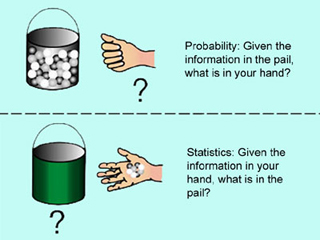
\includegraphics[width=0.8\textwidth, trim={0cm, 1cm, 0cm, 1cm}, clip]{prob_stats}}}
%\end{picture}

\end{frame}

%%%%%%%%%%%%%%%%%%%%%%%%%%%%%%%%%%%%%%%%%%%%%%%%%%
\begin{frame}{Binary Relations}
A \bc{binary relation}, $(X, Y, G)$ is an ordered triple where the set $X$ is called the domain, the set $Y$ is called the codomain, and the set G, called the graph, is a subset of the cartesian product of these sets, $G \subseteq X\times Y$.
\bigskip

The graph is a set of ordered pairs, $G = \{(x,y) \ | \ x \in X, y \in Y\}$. If the pair $(x,y) \in G$, we often write $xRy$ and say ``$x$ relates to $y$''. 
\bigskip

When the domain and codomain are the same set, the relation \emph{may} have some of the following interesting properties:

\end{frame}
%%%%%%%%%%%%%%%%%%%%%%%%%%%%%%%%%%%%%%%%%%%%%%%%%%
\begin{frame}{Binary Relations}
\begin{block}{Properties of Relations}
\begin{itemize}
\item[] \bc{Reflexive} if \ \ $\forall x\in X \ \ xRx $
\item[] \bc{Irreflexive} if \ $\forall x \in X \ \ \neg xRx$ 
\item[] \bc{Symmetric} if \ $xRy \implies yRx \ \ \forall x,y\in X$
\item[] \bc{Anti-symmetric} if \ $xRy \wedge  yRx \implies x = y\ \ \forall x,y\in X$
\item[] \bc{Asymmetric} if \ $xRy \implies \neg yRx \ \ \forall x,y\in X$
\item[] \bc{Transitive} if \ $xRy \wedge yRz \implies xRz \ \ \forall x,y,z \in X$
\item[] \bc{Weakly Connected} if \ $xRy \vee yRx \ \ \forall x\not = y \in X$
\item[] \bc{Complete} if reflexive and weakly connected.
\end{itemize}
\end{block}
\bigskip

\begin{exercise}
Consider the game Rock-Paper-Scissors. Let $X = \{R, P, S\}$ and $xRy$ be the relation representing $x$ beats $y$. Which of the above properties does this relation have?
\end{exercise}

\end{frame}
%%%%%%%%%%%%%%%%%%%%%%%%%%%%%%%%%%%%%%%%%%%%%%%%%%
\begin{frame}{Functions}
A \bc{function}, $f$, is a binary relation, $(X, Y, G)$, such that:\\

\begin{center}
	\begin{enumerate}
		\item $\forall x \in X \ \exists y \in Y \ s.t \ (x,y) \in f$
		\item $(x,y)\in G \wedge (x,z) \in G \implies y = z$
	\end{enumerate} 
\end{center}

The \bc{image} of a set $A$ under a function $f$ is the set

\[ f(A) = \{ y \in Y \ | \ \exists x \in A \text{ s.t. } f(x) = y\}\]


The \bc{pre-image} of a set $B$ under a function $f$ is the set
\[ f^{-1}(B) = \{x \in X \ | \ f(x) \in B\} \]

The \bc{range} of a function, $im(f)$,  is the image of its domain.
\end{frame}

%%%%%%%%%%%%%%%%%%%%%%%%%%%%%%%%%%%%%%%%%%%%%%%%%%
\begin{frame}{Functions}

\begin{figure}[t]
	\centering
	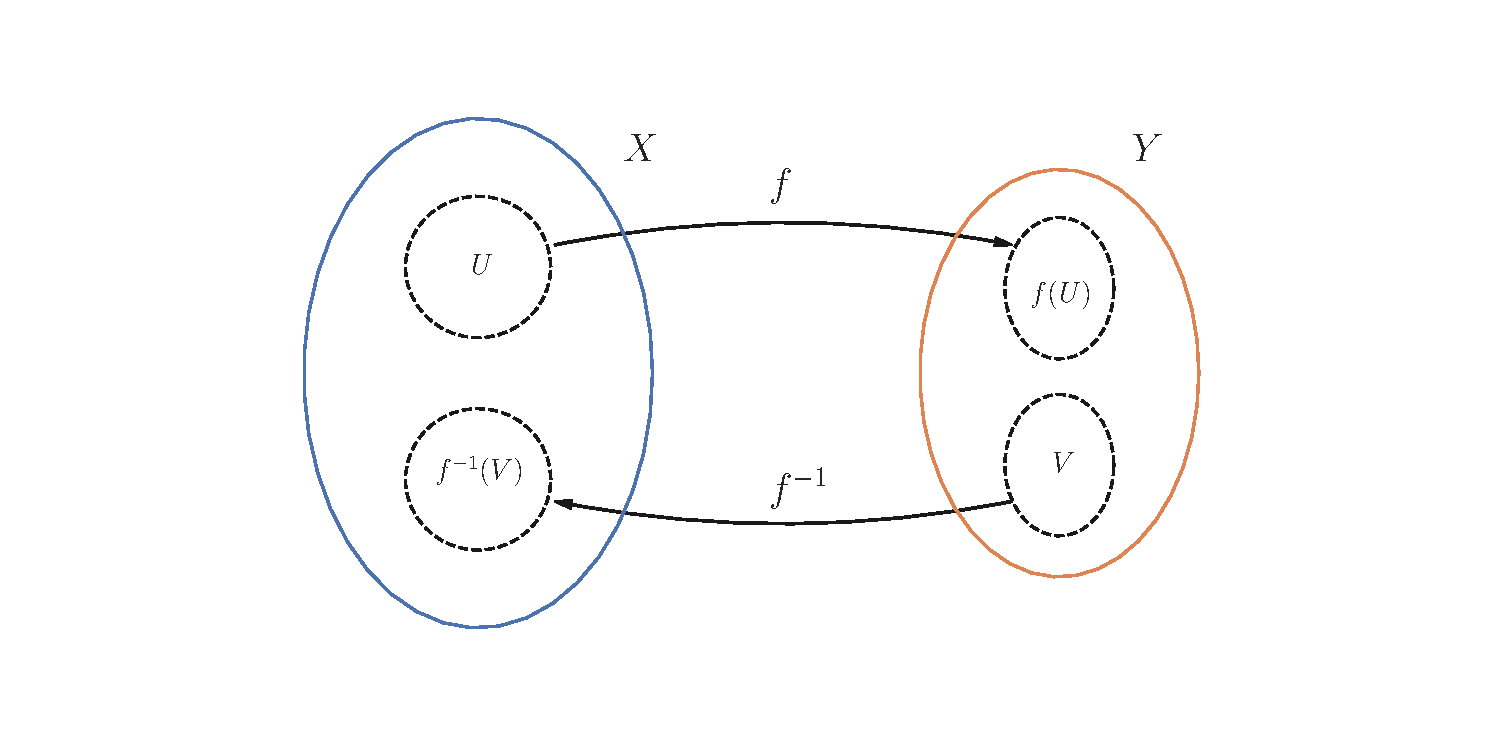
\includegraphics[width=0.8\textwidth]{functions.pdf}
\end{figure}

A function $f:X\into Y$ is said to be an 
\begin{itemize}
\item[] \bc{Injection} (one-to-one) if \ $f(a) = f(b) \implies a = b \ \ \forall a,b \in X$
\item[] \bc{Surjection} (onto) if \ $\forall y\in Y \ \exists x \in X \ s.t \ f(x) = y$
\item[] \bc{Bijection} if it is both injective and surjective
\end{itemize}
\bigskip

Functions that are bijective have an \bc{inverse function}.
\end{frame}
%%%%%%%%%%%%%%%%%%%%%%%%%%%%%%%%%%%%%%%%%%%%%%%%%%
\begin{frame}{Functions}
\begin{exercise}
\begin{enumerate}[a)]
	\item Show that the composition of two bijetive functions is bijective.
	\item Over what subset of $\R$ does $f(\theta) = \sin \theta$ have an inverse?
\end{enumerate}
\end{exercise}
\vfill\vfill 

\bigskip\vfill\vfill
\end{frame}

%%%%%%%%%%%%%%%%%%%%%%%%%%%%%%%%%%%%%%%%%%%%%%%%%%
\begin{frame}{Metric Spaces}
A \bc{metric space} is a pair $(X,d)$ where $X$ is a set and\\ $d:X\times X \rightarrow \R$ is a function which satisfies the following conditions
\begin{enumerate}
\item $d(x,y) \geq 0 \ \  \forall x,y\in X \text{  and  } d(x,y) = 0 \Leftrightarrow x = y$

\item $d(x,y) = d(y,x) \ \ \forall x,y \in X$

\item $d(x,z) \leq d(x,y) + d(y,z) \quad \forall x,y,z \in X \ \ \text{(\emph{Triangle inequality})}$

\end{enumerate}
\bigskip

One advantage of being able to talk about distance is that we could define \bc{continuity} for functions:\bigskip

\bc{$\epsilon - \delta$ Continuity} \\
$\forall \epsilon > 0 \ \ \exists \delta > 0 \ \ s.t \ \ d(x,c)<\delta \implies d\left(f(x), f(c)\right) < \epsilon$
\bigskip

\end{frame}

%%%%%%%%%%%%%%%%%%%%%%%%%%%%%%%%%%%%%%%%%%%%%%%%%%
\begin{frame}{Open Sets}
It was sometimes useful to talk about all the points \emph{within} some distance of another point.\bigskip


An \bc{open ball} of radius $\epsilon > 0$ centered at $a$ is the set:

\[ B(a,\epsilon) = \{x \in X\ | \ d(x,a) < \epsilon\}\]
\bigskip

We defined a set to be \bc{open} if every point had a little neighborhood it could move around in and stay inside the set:

\[\forall x \in X \quad \exists \epsilon > 0 \ \ s.t \ \ B(x,\epsilon) \subseteq X\]
\bigskip

A set $X$ is \bc{closed} if its complement is open.\bigskip
\vfill
\end{frame}

%%%%%%%%%%%%%%%%%%%%%%%%%%%%%%%%%%%%%%%%%%%%%%%%%%
\begin{frame}{Open Sets}

One strategy for showing that a particular set is open (closed) is to show that you can place an open ball around any point in the set (set's complement) that's contained in the set (complement).\bigskip

Another was to exploit some useful properties:

\begin{block}{}
\begin{itemize}
	\item The union of any collection of open sets is open.
	\item The intersection of any collection of closed sets is closed.
		\smallskip
	\item The intersection of a finite collection of open sets is open.
	\item The union of a finite collection of closed sets is closed.
\end{itemize}
\end{block}
\bigskip

\begin{exercise}
Show that the closed ring centered at the origin, $\{x \in \R^{2} \ | \ r \leq d(0, x) \leq R\}$, is a closed set. 
\end{exercise}
\end{frame}
%%%%%%%%%%%%%%%%%%%%%%%%%%%%%%%%%%%%%%%%%%%%%%%%%%
\begin{frame}{Sequences}

A \bc{sequence} is a function whose domain is the natural numbers.\bigskip

A sequence, $\{x_{n}\}_{n \in \N}$, is said to \bc{converge} to a point $a$ if

\[\forall \epsilon > 0 \quad \exists N\in \N \ \ s.t \ \ \forall n > N \ \  d(x_{n}, a) < \epsilon\]
\bigskip

or in other  words:\bigskip

Every $\epsilon$-ball centered at $a$ must contain \textit{all but finitely many} elements of the sequnce.

\end{frame}

%%%%%%%%%%%%%%%%%%%%%%%%%%%%%%%%%%%%%%%%%%%%%%%%%%
\begin{frame}{Convergence of Sequences}
Hypothesizing that a sequence converges to a particular point $a$ and showing that the definition is satisfied is one strategy for proving convergence. But we had some shortcuts:\bigskip

\begin{theorem}[Monotone Convergence Theorem]
A monotone sequence of real numbers converges iff it is bounded.\\

Further, if it is increasing (resp. decreasing), it converges to its supremum (infimum).
\end{theorem}
\end{frame}
%%%%%%%%%%%%%%%%%%%%%%%%%%%%%%%%%%%%%%%%%%%%%%%%%%
\begin{frame}{Convergence of Sequences}

A sequence $\{x_{n}\}$ is called a \bc{Cauchy sequence} if:

\[ \forall \epsilon > 0 \ \exists N\in \N \text{ s.t. } \forall m,n > N \ d(x_{m}, x_{n}) < \epsilon\]
\bigskip

\begin{theorem}[Cauchy Convergence Criterion]
A sequence of real numbers is convergent iff it is Cauchy
\end{theorem}

\begin{exercise}
Show that the sequence $x_{0} = 100$, $x_{k+1} = \sqrt{x_{k}}$ is convergent.
\end{exercise}
\end{frame}

%%%%%%%%%%%%%%%%%%%%%%%%%%%%%%%%%%%%%%%%%%%%%%%%%%
\begin{frame}{Completeness}

It would be very convenient if every Cauchy sequence were convergent. Such a metric space is said to be \bc{complete}.\bigskip

What conditions are sufficient to ensure this?\bigskip

Maybe closedness? We know the following property of closed sets\bigskip

\begin{block}{Proposition: Closed sets contain their limit points}
Let $(X, d)$ be a metric space. If $A\subseteq X$ is a closed subset and $a_{n}\in A$ is a sequence, then
$$a_{n} \rightarrow a \implies a \in A$$
\end{block}\bigskip

But we saw that that wasn't enough (e.g., sequnce of rationals converging to $\sqrt{2}$).
\end{frame}

%%%%%%%%%%%%%%%%%%%%%%%%%%%%%%%%%%%%%%%%%%%%%%%%%%
\begin{frame}{Compactness}

A set is \bc{compact} if \emph{every} open cover has a finite sub-cover. \bigskip

That does the trick, and a few others:

\begin{block}{}
	\begin{itemize}
		\item A compact metric space is complete.
		\item A closed subset of a compact set is compact.
		\item A compact subset of $R$ has a maximum and minimum value.
	\end{itemize}
\end{block}

\bigskip

In $\R^{n}$, the Heine-Borel theorem tells us that the compact sets are ones that are \bc{closed} and \bc{bounded}.
\end{frame}

%%%%%%%%%%%%%%%%%%%%%%%%%%%%%%%%%%%%%%%%%%%%%%%%%%
\begin{frame}{Compactness}
With these concepts, we saw how they applied to micro theory, particularly representing preferences and showing that utility maximization problems had solutions.\bigskip

We also got a powerful fixed point theorem that would later show up in dynamic programming.

\begin{theorem}[Banach Fixed-point Theorem]
Let $(X, d)$ be a non-empty complete metric space with a contraction mapping $f:X\to X$. Then $f$ admits a unique fixed-point $x^{*}$, $f(x^{*})=x^{*}$.\medskip

Furthermore, $x^{*}$ can be found by iterating $f$ on an arbitrary initial value. 
\end{theorem}
\bigskip
\end{frame}



%%%%%%%%%%%%%%%%%%%%%%%%%%%%%%%%%%%%%%%%%%%%%%%%%%
\begin{frame}{Linear Algebra}
In linear algebra, we first started out being interested in finding the solutions to a system of linear equation:

\begin{center}
\begin{tabular}{c c c c c c c c c}
$a_{11}x_{11}$   &+&   $a_{12}x_{12}$      &+&    $\cdots$    &+&    $a_{1n}x_{1n}$   &=& $b_1$\\
$a_{21}x_{21}$   &+&   $a_{22}x_{22}$      &+ &   $\cdots$    &+&    $a_{2n}x_{2n}$   &=& $b_2$\\
$a_{31}x_{31}$   &+&   $a_{32}x_{32}$      &+&    $\cdots$    &+&    $a_{3n}x_{3n}$   &=& $b_3$\\
$\vdots$               &+&        $\vdots$                &+&    $\cdots$    &+&    $\vdots$               &=&  $\vdots$\\
$a_{m1}x_{m1}$  &+&   $a_{m2}x_{m2}$   &+&    $\cdots$    &+&    $a_{mn}x_{mn}$ &=& $b_m$
\end{tabular}
\end{center}
\bigskip

which we would represent more conveniently using matrices: $Ax = b$.
\end{frame}

%%%%%%%%%%%%%%%%%%%%%%%%%%%%%%%%%%%%%%%%%%%%%%%%%%
\begin{frame}{Linear Algebra}
We learned a method that works every time for any system:

\begin{center}
\textbf{Recipe for Solving a System of Linear Equations}
\end{center}

\begin{enumerate}[1.]
\item Use row operations to put the augmented system in reduced row echelon form.
\item Is the last column of the augmented system a pivot column? If yes, there is no solution. If no, proceed.
\item Are there any free variables? If no, read the unique solution off of each row. If yes, proceed.
\item Solve for each basic variable in terms of the free variables and a constant. 
\end{enumerate}
\bigskip

The 'put the system in RREF' part, we can make a computer do.
\end{frame}

%%%%%%%%%%%%%%%%%%%%%%%%%%%%%%%%%%%%%%%%%%%%%%%%%%
\begin{frame}{Vector Spaces}
We saw that we could get some powerful tools if we thought about matrices as functions. But functions of what?\bigskip

A \bc{vector space} is a structure formed by a set $V$ (whose elements are called vectors) together with two operations: addition and scalar multiplication.\bigskip

\begin{block}{Vector space axioms}
\begin{enumerate}
\item \emph{Commutativity of vector addition} \quad $\x + \y = \y + \x$

\item \emph{Associativity of vector addition} \quad $(\x + \y) + \z = \x + (\y + \z)$

\item \emph{Additive identity:} There is a $\mathbf{0}$ s.t \quad $\mathbf{0} + \x = \x $

\item \emph{Additive inverse:} $\forall \x$ there exists a $-\x$ s.t \quad $\x + -\x = \mathbf{0}$

\item \emph{Associativity of scalar multiplication} \quad $r(s\x) = (r s)\x$

\item \emph{Distributivity of scalar sums} \quad $ (r + s) \x = r\x + s\x$

\item \emph{Distributivity of vector sums} \quad $r(\x + \y) = r\x + r\y$

\item \emph{Scalar identity} \quad $1\cdot \x = \x$

\end{enumerate}
\end{block}
\end{frame}

%%%%%%%%%%%%%%%%%%%%%%%%%%%%%%%%%%%%%%%%%%%%%%%%%%
\begin{frame}{Linear Independence and Span}
Now that we can add and scalar multiply the elements of our set, there are new properties we can talk about:

The vectors $v_1,\dots,v_n$ are \bc{linearly independent} if, for scalars $c_1,\dots,c_n \in \R$, the only solution to the equation
\[c_1v_1 + \dots + c_n v_n = 0\]

The vectors $v_1,\dots,v_n$ are \bc{spanning} if for every vector $v\in V$, we can find $c_1, \dots, c_n \in \R$ such that
\[v = c_1 v_1 + \dots + c_n v_n\]

In which case we may write $V = \text{span}\{v_1,\dots,v_n\}$.
\end{frame}

%%%%%%%%%%%%%%%%%%%%%%%%%%%%%%%%%%%%%%%%%%%%%%%%%%
\begin{frame}{Linear Independence and Span}
How do you check if a set of vectors are linearly independent and spanning?\bigskip

Place the vectors as columns of a matrix: $[v_{1}, \dots, v_{n}]$.\bigskip

Put the matrix in RREF.\bigskip

To check linear independence, check if there are $n$ basic columns.\bigskip

To check spanning, check that every row has a pivot.\bigskip

If the matrix is square, you can do both at once by checking the determinant. \bigskip

The vectors $v_1,\dots,v_n$ form a \bc{basis} for $V$ if they are linearly independent and spanning. \bigskip


A vector space is finite dimensional with dimension $n$ if we can find a vectors $v_1,\dots,v_n \in V$ which form a basis for $V$.\bigskip

\end{frame}

%%%%%%%%%%%%%%%%%%%%%%%%%%%%%%%%%%%%%%%%%%%%%%%%%%
\begin{frame}{Subspaces}
A subset $W \subset V$ is called a \bc{subspace} if and only if

\begin{enumerate}[1.]
\item $\mathbf{0} \in W$
\item If $\mathbf{u},\mathbf{v} \in W$ then $\mathbf{u} + \mathbf{v} \in W$
\item If $\mathbf{u} \in W$ then $\alpha\mathbf{u}\in W$ for any scalar $\alpha \in \R$
\end{enumerate}
\bigskip

\[ \{\x \in \R^{n} \ | \ \x = \mathbf{c} + \v \text{ for some } \v \in V\}\]

is called an \bc{affine subspace} of $\R^{n}$ (but it is not a subspace!).\bigskip


\end{frame}


%%%%%%%%%%%%%%%%%%%%%%%%%%%%%
\begin{frame}{Matrices as Functions}
A function $f:\R^{m}\to\R^{n}$ is a \bc{linear map} if: 
\begin{itemize}
\item $f(x + y) = f(x) + f(y)$ \ $\forall x,y\in V$.
\item $f(\alpha x) = \alpha f(x)$ \ $\forall \alpha \in \R, \ x \in V$.
\end{itemize}
\bigskip

\begin{block}{Proposition}
Let $f:\R^{m}\to\R^{n}$ be a linear map. Further, let the vectors of $\R^{m}$ and $\R^{n}$ be column vectors. Then there exists a matrix $A$ such that
\[f(\v)\ = A\v\]
\end{block}
\bigskip

\begin{exercise}
Consider the function which takes a vector in $\R^{2}$ and returns its mirror image about the y-axis. Is this a linear mapping? What matrix corresponds to it?
\end{exercise}
\end{frame}

%%%%%%%%%%%%%%%%%%%%%%%%%%%%%
\begin{frame}{Matrices as Functions}
If matrices are linear functions, do we have analogues of the image, zeros, and fixed points?\bigskip

Yes, and these are subspaces!\bigskip

The image of a matrix is its \bc{column space}, $\text{Col}(A) = \{b \in \R^{n} \ | \ Ax = b \ \text{for some }x\}$.\bigskip

The set of zeros of a matrix is its \bc{null space}, $\text{Null}(A) = \{x \in \R^{n} \ | \ Ax = 0\}$.\bigskip

The rank-nullity theorem connects these and the total number of columns, $n$,  by:

\[\text{dim Col}(A) + \text{dim Null}(A) = n\]
\end{frame}

%%%%%%%%%%%%%%%%%%%%%%%%%%%%%
\begin{frame}{Solutions to Systems Again}

\begin{theorem}
If $\mathcal{S}$ is non-empty, such that there is at least one particular solution, $\x^{*}$, such that $A\x^{*} = \b$. Then $\mathcal{S}$ is the affine subspace

\[\mathcal{S} = \{\x^{*} + \v \ | \ \v \in \text{Null}(A)\}\]
\end{theorem}

\begin{exercise}
Find the solutions to the augmented system
\[ \begin{pmatrix}1 & 0 & 2\\ 0 & 1 & 0 \\ 0 & 0 & 0 \end{pmatrix} x = \begin{bmatrix}1 \\ 2 \\ 0 \end{bmatrix}\]

Show that the solution set is an affine subspace.
\end{exercise}

\end{frame}

%%%%%%%%%%%%%%%%%%%%%%%%%%%%%
\begin{frame}{Eigenvalues and Eigenvectors}
For the analogue of fixed points we have:\bigskip


Let $A:\R^{n}\to\R^{n}$ be a linear map. An \bc{eigenvector} $\v$ of $A$ and its corresponding \bc{eigenvalue}, $\lambda$, are a vector and scalar satisfying 
\[ A\v = \lambda\v\]
\bigskip

We can find the eigenvalues by solving:
\[\det(\lambda \mathbf{I} - A) = 0\]\bigskip

We can solve for the eigenvectors by solving the augmented system;

\[\left(\lambda I - A \ | \  0 \right)\]

for each $\lambda$. For small  systems we can use the trick $tr(A) = \sum \lambda_{i}$ and $det(A) = \Pi \lambda_{i}$.
\end{frame}

\begin{frame}{Diagonalization}
\begin{theorem}
Let $A$ be an $n\times n$ matrix. Let $\lambda_1,\dots,\lambda_n$ be eigenvalues of $A$ with corresponding eigenvectors $\v_1,\dots,\v_n$. Construct the matrix
\[P = [\v_1, \dots, \v_n]\]
whose columns are $A$'s eigenvectors. If $P$ in invertible, then
\[ P^{-1}AP = 
\left (
\begin{array}{c c c c }
\lambda_1 & 0 & \cdots & 0\\
0 & \lambda_2 & \cdots & 0\\
\vdots & \vdots & \cdots & \vdots\\
0 & 0 & 0 & \lambda_n
\end{array}
\right )
\]
\end{theorem}
\end{frame}
%%%%%%%%%%%%%%%%%%%%%%%%%%%%%%%%%%%%%%%%%%%%%%%%%%%%%
\begin{frame}{Diagonalization}
\begin{theorem}[The Spectral Theorem]
Let $A$ be an $n\times n$ matrix of real entries that is symmetric (i.e., $A^{\prime} = A$). Then $A$ can be diagonalized 

\[A = Q D Q^{\prime}\]

where $Q$ is an orthogonal matrix ($Q^{-1} = Q^{\prime}$).
\end{theorem}
\end{frame}
%%%%%%%%%%%%%%%%%%%%%%%%%%%%%%%%%%%%%%%%%%%%%%%%%%%%%
\begin{frame}{Diagonalization}

We saw how we can use this property to solve homogeneous first-order difference equations, $\mathbf{x_{t+1}} = A \mathbf{x}_{t}$. 

\[\mathbf{x}_t = c_1 \lambda_1^t \mathbf{v}_1 + \dots + c_n \lambda_n^t \mathbf{v}_n\]
\end{frame}
%%%%%%%%%%%%%%%%%%%%%%%%%%%%%%%%%%%%%%%%%%%%%%%%%%%%%

\begin{frame}{Quadratic Forms}

\[\mathcal{Q}(x_{1},x_{2},\dots, x_{n}) = \sum_{i \leq j} a_{ij}x_{i}x_{j}\]
\bigskip

Any quadratic form can be written more compactly as
\bigskip

\[\mathcal{Q}(x_{1},\dots,x_{n}) = \x^{'}A\x\]
\bigskip

where $A$ is a unique real-valued symmetric matrix.

\end{frame}

%%%%%%%%%%%%%%%%%%%%%%%%%%%%%%%%%%%%%%%%%%%%%%%%%%%%%

\begin{frame}{Quadratic Forms}
\begin{figure}
	\begin{subfigure}[b]{0.45\textwidth}
		\centering
		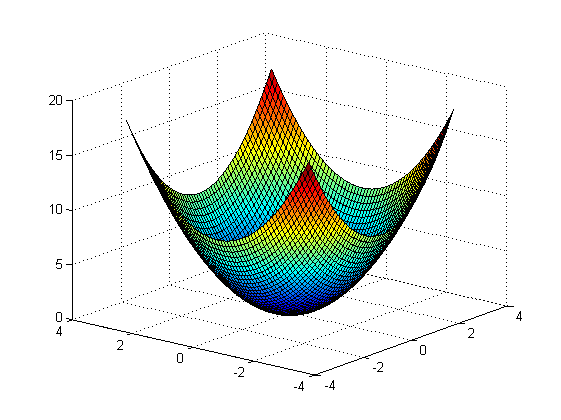
\includegraphics[width=\textwidth]{quadraticform1}
	\end{subfigure}
	\begin{subfigure}[b]{0.45\textwidth}
		\centering
		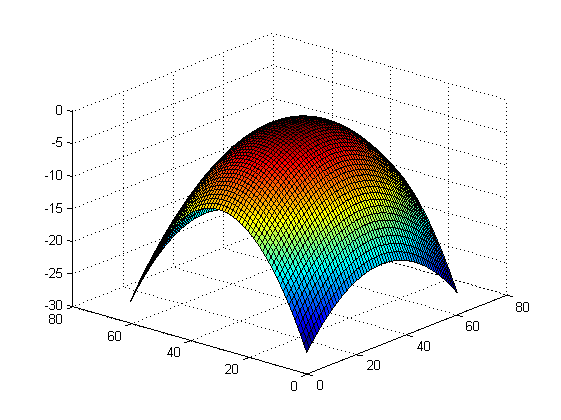
\includegraphics[width=\textwidth]{quadraticform2}
	\end{subfigure}

	\begin{subfigure}[b]{0.45\textwidth}
		\centering
		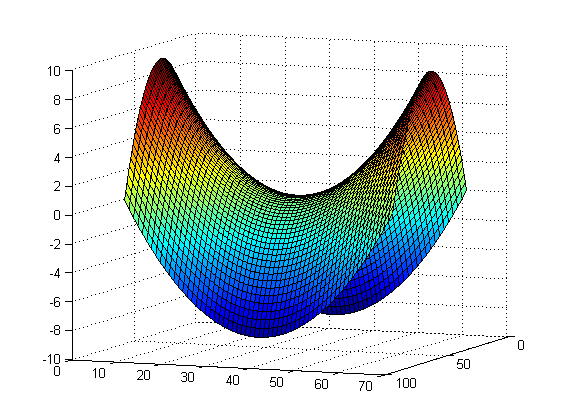
\includegraphics[width=\textwidth]{quadraticform3}
	\end{subfigure}
	\begin{subfigure}[b]{0.45\textwidth}
		\centering
		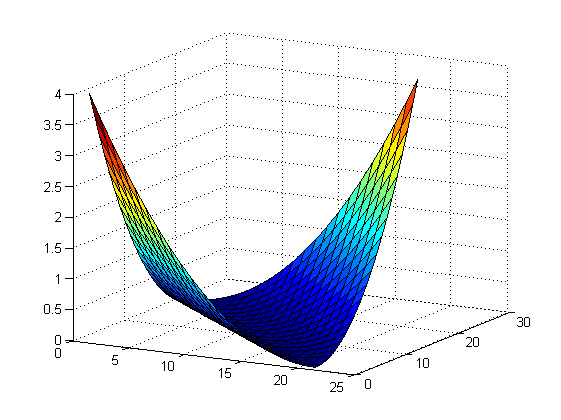
\includegraphics[width=\textwidth]{quadraticform4}
	\end{subfigure}

\end{figure}
\end{frame}

%%%%%%%%%%%%%%%%%%%%%%%%%%%%%%%%%%%
\begin{frame}{Definiteness}
\begin{theorem}
Let $A$ be a symmetric matrix. Then
\begin{enumerate}[a)]
\item $A$ is positive definite iff all eigenvalues are $> 0$.
\item $A$ is negative definite iff all eigenvalues are $< 0$.
\item $A$ is positive semidefinite iff all eigenvalues are $\geq 0$.
\item $A$ is negative semidefinite iff all eigenvalues are $\leq 0$
\item $A$ is indefinite iff it has at least one positive and one negative eigenvalue.  

\end{enumerate}
\end{theorem}
\end{frame}

%%%%%%%%%%%%%%%%%%%%%%%%%%%%%
\begin{frame}{Axioms of Probability}
A \textbf{probability} is a function, $\P : 2^{\Omega} \to [0, 1]$ such that
\begin{enumerate}[1.]
\item $0 \leq \P(E) \leq 1$
\item $\P (\Omega) = 1$
\item For any countable sequence of \emph{disjoint} events $E_{i}$,
\[\P\left (\bigcup_{i=1}^{\infty} E_{i} \right) = \sum_{i=1}^{\infty} \P(E_{i}) \]
\end{enumerate}
\vfill

Probability \emph{measures} the size of sets in a particular way.

\vfill
\small
NB: This is not entirely correct. The domain of the function is not the whole power set but a subset that is a ``measurable space'' and $\P$ must be a ``measurable function'', but this is beyond our scope.
\end{frame}

%%%%%%%%%%%%%%%%%%%%%%%%%%%%%
\begin{frame}{Properties of Probability}

Let $A$ and $B$ be events. The probability of $A$ \bc{conditional} on having observed $B$ is 
\[ \P(A|B) = \frac{\P(A \cap B)}{\P(B)}\]
\bigskip

Two events $A$ and $B$ are said to be \bc{independent} if 

\[\P(A \cap B) = \P(A)\cdot \P(B)\]
\bigskip

The \bc{law of total probability}: 
\[\P(A) = \sum_{i=1}^{n} \P(A|B_{i}) \P(B_{i})\]

and \bc{Bayes' theorem}
\[ \P(A | B) = \frac{\P(B | A) \P(A)}{\P(B)}\]

\end{frame}

\begin{frame}{Expectation}
Rather than dealing with outcomes, we want to deal with \bc{random variables}, $f:\Omega \to \R$.

\[ \E[X] = \sum_{x} x\cdot \P(x) \]


\[ \E[X] = \int_{-\infty}^{\infty} x f(x) \mathrm{d}x \]

\vfill
For this to be well defined, we require that $\E[|X|] < \infty$.
\end{frame}

%%%%%%%%%%%%%%%%%%%%%%%%%%%%%
\begin{frame}{Moments}

The $k$-th \bc{central moment} is defined as 

\[\mu_{k} = \E[(X - \E[X])^{k}]\]\bigskip

The $k$-th \bc{raw moment} is defined as 

\[\mu_{k}^{\prime} = \E[X^{k}]\]\bigskip

The \bc{variance} is the second central moment. 
\end{frame}

%%%%%%%%%%%%%%%%%%%%%%%%%%%%%
\begin{frame}{Moment Generating Functions}

If all of the moments exist, we can talk about the \bc{moment generating function}.

\[M_{X}(t) = \E[e^{tX}]\]

\bigskip

The MGF has the following useful properties:
\begin{enumerate}
	\item If random variables $X$ and $Y$ have the same MGF, they have the same distribution.
	\item If $X$ and $Y$ are independent random variables, then their sum $X + Y$ has MGF: $M_{X+Y}(t) = M_{X}(t) \cdot M_{Y}(t)$.
	\item $M_{cX}(t) = M_{X}(ct)$.
	\item $\mu_{k}^{\prime} = \left. \frac{\mathrm{d}^{n}M_{X}}{\mathrm{d}t^{n}}\right\vert_{t=0}$
\end{enumerate}
\end{frame}

%%%%%%%%%%%%%%%%%%%%%%%%%%%%%
\begin{frame}{Jointly Distributed Random Variables}
\[ F(a,b) = \P(X \leq a, Y \leq b) \quad \ -\infty < a,b < \infty\]

\[\mathrm{Cov}(X,Y) = \E[XY] - \E[X]\E[Y]\]

We get \bc{correlation} by scaling covariance by the appropriate variances.

\[\mathrm{Corr}(X, Y) = \frac{\mathrm{Cov}(X, Y)}{\sqrt{\mathrm{Var}(X)\mathrm{Var}(Y)}}\]
\end{frame}

%%%%%%%%%%%%%%%%%%%%%%%%%%%%%
\begin{frame}{Properties of Multivariate Normal}

\begin{block}{Proposition}
Let $\x \sim N(\mathbf{\mu}, \mathbf{\Sigma})$. Then for some non-zero matrix $A$ (or vector) we have
\[ \mathbf{A}\x \sim N(\mathbf{A}\mathbf{\mu}, \mathbf{A} \mathbf{\Sigma} \mathbf{A}^\prime)\]
\end{block}

\begin{theorem}
Let $\x \sim N(\mathbf{0}, \sigma^2\mathbf{I})$ and let $M$ be a symmetric idempotent matrix of rank $m$. Then
\[\frac{\x^\prime M \x}{\sigma^2} \sim \chi^2(m)\]
\end{theorem}

\end{frame}

\begin{frame}{Inequalities}
\begin{theorem}[Markov's Inequality]
If X is a random variable that takes only nonnegative values, then for any value $a > 0$
\[\P(X \geq a) \leq \frac{\E[X]}{a}\]
\end{theorem}

\begin{theorem}[Chebyshev's Inequality]
If X is a random variable with mean $\mu$ and variance $\sigma^{2}$, then for any $\epsilon > 0$
\[\P(|X - \mu| > \epsilon) \leq \frac{\sigma^{2}}{\epsilon^{2}}\]
\end{theorem}

\begin{theorem}[Jensen's Inequality]
Let $X$ be a random variable and $f(\cdot)$ be a convex function. Then
\[f(\E[X]) \leq \E[f(X)]\]
\end{theorem}

\end{frame}

%%%%%%%%%%%%%%%%%%%%%%%%%%%%%%%%%%%%%%%%%%%%%%%%

\begin{frame}{Estimation}

Let $F$ be a distribution with parameter $\theta$. An \bc{estimator} is a function of a sample from $F$.

\[\hat{\theta} = T(X_1, \dots, X_n; F)\]
\bigskip

An estimator is \bc{unbiased} if $\E [ \hat{\theta} ]  = \theta$.\bigskip
\bigskip

An estimator, $\hat{\theta}$, is \bc{consistent} for a parameter $\theta$ if $\hat{\theta} \overset{p}{\to} \theta$.

\end{frame}

%%%%%%%%%%%%%%%%%%%%%%%%%%%%%
\begin{frame}{Convergence of Random Variables}
We had some different modes of convergence for random variables:

$\{X_{n}\}$ \bc{converges in probability} to $X$, if $\forall \epsilon > 0 \ \lim_{n\to\infty} \P(  |X_{n} - X| > \epsilon) = 0$.
\bigskip

$\{X_{n}\}$ \bc{converges almost surely} to $X$,  if $ \P( \lim_{n\to\infty} X_{n} = X) = 1$.
\bigskip

$\{X_{n}\}$ \bc{converges in distribution} to $X$, if $F_{n}(x) \to F(x) \quad \forall x$. 
\bigskip

Convergence almost surely $\implies$ convergence in probability $\implies$ convergence in distribution

\end{frame}

%%%%%%%%%%%%%%%%%%%%%%%%%%%%%
\begin{frame}{Convergence of Random Variables}
\begin{theorem}[Continuous Mapping Theorem]
Let $g(\cdot)$ be a continuous function. Then for $i \in \{d, p, a.s.\}$
\begin{align*}
& X_{n} \overset{i}{\to} X \implies g(X_{n}) \overset{i}{\to} g(X)\\	
\end{align*}
\end{theorem}

\begin{theorem}[Slutsky's Theorem]
Let $X_{n} \overset{d}{\to} X$ and $Y_{n} \to c$.
\begin{align*}
&X_{n} + Y_{n} \overset{d}{\to} X + c\\
& X_{n}Y_{n} \overset{d}{\to} Xc\\
& X_{n}/Y_{n} \overset{d}{\to} X / c, \text{provided $c \not \to 0$ }.
\end{align*}
\end{theorem}
\end{frame}

%%%%%%%%%%%%%%%%%%%%%%%%%%%%%
\begin{frame}{Limit Theorems}
We frequently appeal to one of the following (family of ) laws:

\begin{theorem}[law of large numbers]
Let $X_{1}, \dots, X_{n} \sim F$ be an iid sample from a distribution with mean $\mu$. 
\[\bar{X}_{n} = \frac{1}{n}\sum X_{i} \overset{p}{\to} \mu\]
\end{theorem}

\begin{theorem}[Central Limit Theorem]
Let $X_{1}, \dots X_{n} \overset{iid}{\sim} F$, with $\E[X] = \mu$ and $\mathrm{Var}(X) = \sigma^{2}$, both finite. Let $\bar{X}_{n} = \frac{1}{n}\sum X_{i}$. 

\[\sqrt{n} (\bar{X}_{n} - \mu) \overset{d}{\to} N(0,\sigma^{2})\]
\end{theorem}
\end{frame}

\begin{frame}{Limit Theorems for Random Vectors}

\begin{theorem}[Multivariate CLT]
Suppose $\X$ is a random vector with finite mean $\mathbf{\mu}$ and variance $\mathbf{\Sigma}$. Then
\[ \sqrt{n} \left ( \bar{\X}_n - \mathbf{\mu}\right) \overset{d}{\rightarrow} N(\mathbf{0}, \mathbf{\Sigma})\]
\end{theorem}
\bigskip


Using Slutsky's theorem, if $\mathbf{A}_{n} \overset{p}{\to} A$ then $\sqrt{n} \mathbf{A}_{n} \left ( \bar{\X}_n - \mathbf{\mu}\right) \overset{d}{\rightarrow} N(\mathbf{0}, \mathbf{A}\mathbf{\Sigma}\mathbf{A}^{\prime})$.
\end{frame}

%%%%%%%%%%%%%%%%%%%%%%%%%%%%%
\begin{frame}{Taylor Series}
Smooth functions admit a Taylor series.

\[f(x) = \sum_{n = 0}^{\infty} \frac{f^{(n)}(a)}{n!}\left(x-a\right)^{n}\]

We can use a few terms of the series and be confident our error is small if we're close to the point we expanded the series around.

\begin{theorem}
Let $f:\R\into\R$ be $k$ times differentiable at the point $a\in\R$. Then there exists a function $R_{k}:\R\into\R$ such that

\[f(x) = f(a) + f^{'}(a)\left (x-a\right) + \frac{f^{''}(a)}{2}\left(x-a\right)^{2} + \dots + \frac{f^{(k)}}{k!} \left(x-a\right)^{k} + R_{k}(x)\]
such that
\[lim_{x\to a} R_{k}(x)/x^{k} = 0\]
\end{theorem}
\end{frame}

%%%%%%%%%%%%%%%%%%%%%%%%%%%%%
\begin{frame}{Multivariate Functions}


A \bc{level set} of a function $f:\R^{n}\into \R$ is the set

\[ \mathcal{L} = \{\x \in \R^{n} \ | \ f(\x) = c  \} \]

for some $c \in \R$.\bigskip

The \bc{gradient} is the vector of partial derivatives: 

\[\nabla f(\x) = \left (\frac{\partial f}{\partial x_{1}}, \frac{\partial f}{\partial x_{2}},\dots, \frac{\partial f}{\partial x_{n}}   \right ) \]
\bigskip 

At any point, the tangent to the level set and the gradient vector are orthogonal.

\end{frame}

%%%%%%%%%%%%%%%%%%%%%%%%%%%%%%%%%%%%%%%%%%%%%%%
\begin{frame}{Log-linearization}

In log-linearizing an equation, we want to transform it from being in levels to being in percentage deviation from the steady state

\[\hat{x}_{t} = \frac{x_{t} - \bar{x}}{\bar{x}}\]
\bigskip

For most equations, we won't be able to write it like this exactly. We'll need to write it approximately:

\begin{align*}
f(x_{t}) &\approx f(\bar{x}) + f^{\prime}(\bar{x}) (x_{t} - \bar{x})\\
&= f(\bar{x}) + f^{\prime}(\bar{x})\bar{x} \hat{x}_{t}
\end{align*}
\end{frame}

%%%%%%%%%%%%%%%%%%%%%%%%%%%%%%%%%%%%%%%%%%%%%%%
\begin{frame}{Unconstrained optimization}

To optimize a function on the interior, set the gradient to zero and solve. $\nabla f(x^{*}) = 0$.\bigskip
\bigskip

Construct the Hessian and check it's negative (positive) definite for a local maximum (minimum).

\end{frame}

%%%%%%%%%%%%%%%%%%%%%%%%%%%%%%%%%%%%%%%%%%%%%%%%%%%%%%%%
\begin{frame}{Equality Constrained Optimization}
Consider the optimisation problem

\begin{align*}
\underset{\{x_{1}, x_{2}\}}{\mathrm{max}}  \quad& f(x_{1}, x_{2})\\
\text{s.t}\quad \ \ & g(x_{1}, x_{2}) = h
\end{align*}

To determine what conditions might be necessary for an optimum, consider these functions and their level sets.

\begin{figure}
	\begin{subfigure}[b]{0.45\textwidth}
		\centering
		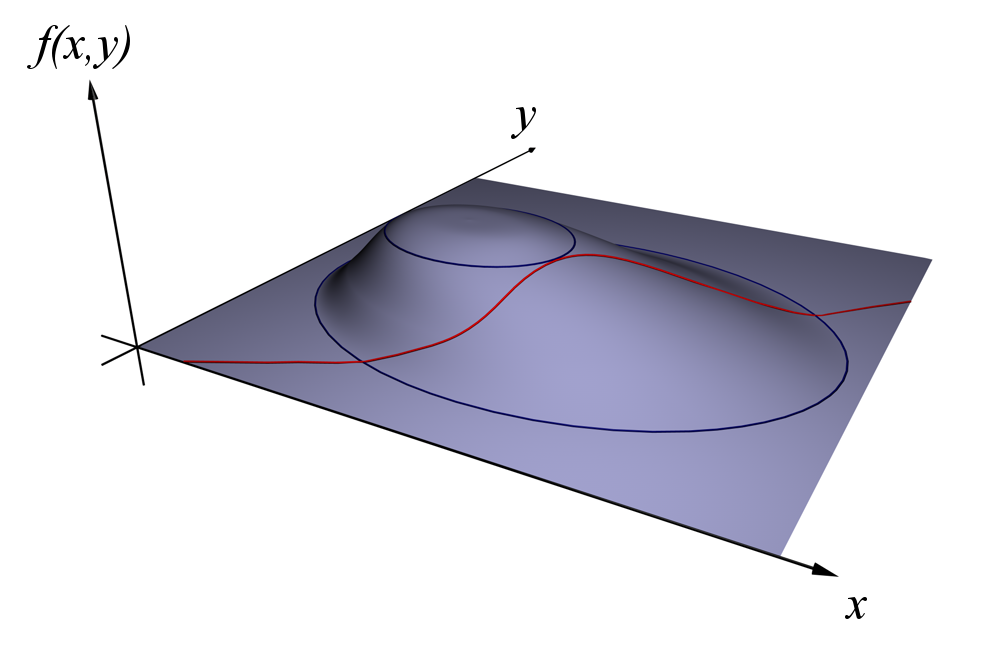
\includegraphics[width=\textwidth]{LagrangeMultipliers3D.png} 
	\end{subfigure}\hfill
	\begin{subfigure}[b]{0.45\textwidth}
		\centering
		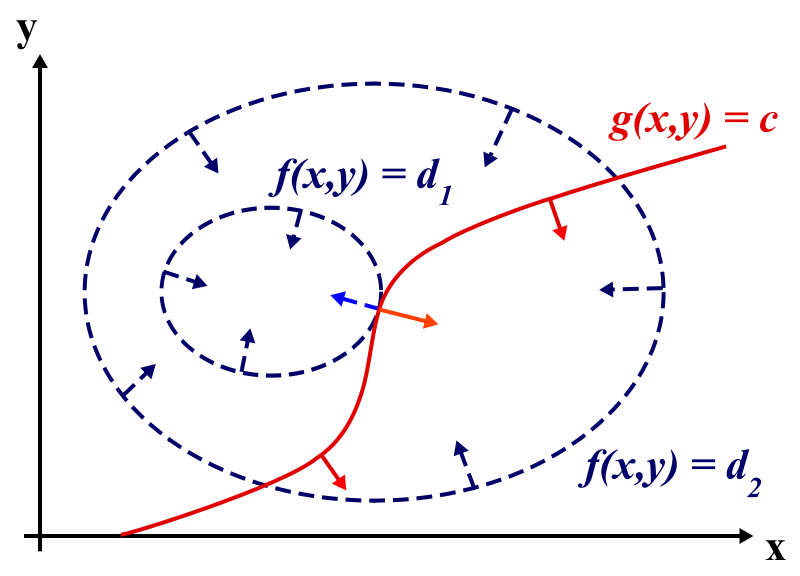
\includegraphics[width=\textwidth]{LagrangeMultipliers2D.png} 
	\end{subfigure}\hfill
\end{figure}

\end{frame}

%%%%%%%%%%%%%%%%%%%%%%%%%%%%%%%%%%%%%%%%%%%%%%%%%%%%%%%%
\begin{frame}{Equality Constrained Optimization}
At an optimum, the level set of the function and the constraint set are tangent. \\

\[\nabla f(\x^{*}) = \lambda \nabla g(\x^{*})\]
\smallskip

However, for $\lambda$ to be uniquely defined, we need to require that $\nabla g(\x^{*}) \not = 0$.

Construct the Lagrangian

\[\mathcal{L} = f(x) + \lambda [h - g(x)]\]

Solve this unconstrained problem, $\nabla \mathcal{L} = 0$.

\end{frame}

%%%%%%%%%%%%%%%%%%%%%%%%%%%%%%%%%%%%%%%%%%%%%%%%%%%%%
\begin{frame}{Inequality Constrained Optimization}

Consider the problem with one inequality constraint 

\begin{align*}
\underset{\{x_{1}, x_{2}\}}{\mathrm{max}}  \quad& f(x_{1}, x_{2})\\
\text{s.t}\quad \ \ & g(x_{1}, x_{2}) \leq h
\end{align*}

As before, it'll be necessary that at a local max/min, $\x^{*}$
\[\nabla f(\x^{*}) = \mu \nabla g(\x^{*})\]\bigskip

But this time we can't take partials with respect to Lagrange multipiliers (that gives us binding constraints). Instead we use the conditions:

\[g((x) \leq h \qquad \mu\geq 0 \qquad \mu [h-g(\x)^{*}] = 0\]

\end{frame}

%%%%%%%%%%%%%%%%%%%%%%%%%%%%%%%%%%%%%%%%%%%%%%%%%%%%%%%%
\begin{frame}{The Principle of Optimality}

\begin{block}{Principle of Optimality (Bellman, 1957)}
An optimal policy has the property that whatever the initial state and initial decision are, the remaining decisions must constitute an optimal policy with regard to the state resulting from the first decision.
\end{block}
\bigskip

Tells us to look for a recursive formulation of the problem.\bigskip

\[V(k_{t}) = \underset{c_{t}}{\max} \quad \left\{U(c_{t}, k_{t}) + \beta V(g(c_{t}, k_{t})) \right\}\]
\bigskip

This is not a sequence problem but a \bc{functional equation} problem. The solution is a pair of functions: $\sigma(k_{t})$ and $V(k_{t})$.

 \vfill\vfill
\end{frame}

\begin{frame}{Properties (Stokey, Lucas, Prescott)}
If 
\begin{enumerate}[{A}1.]
\item The constraint set $\{x \ | \ x = g(c_{t}, k_{t})\}$ is non-empty for all $k_{t}$.
\item The constraint set is compact and $f(\cdot)$ and $g(\cdot)$ are continuous.
\item $f(\cdot)$ is strictly concave. The constraint set is convex. 
\item $f(\cdot)$ is strictly increasing.
\item $f(\cdot)$ is $\mathcal{C}^{1}$ on the interior of its domain.
\end{enumerate}
\bigskip

then there are unique value and policy functions that solve the problem, and the solution is identical to the sequence problem's solution. The value function is strictly increasing, strictly concave, continuous, and differentiable. 
\end{frame}

%%%%%%%%%%%%%%%%%%%%%%%%%%%%%%%%%%%%%%%%%%%%%%%%%%%%%%%%
\begin{frame}{The Bellman Operator}
Define the operator $T:X\to X$ (where $X$ is a function space) to be:
\[T(V) = \underset{c}{\max}\left\{ f(c, k) + \beta V( g(c,k))  \right\} \]
\bigskip

The value function we're looking for is a fixed point of this operator

\[T(V) = V\]

\end{frame}

%%%%%%%%%%%%%%%%%%%%%%%%%%%%%%%%%%%%%%%%%%%%%%%%%%%%%%%%
\begin{frame}{Contraction Mapping}
\begin{theorem}[Blackwell's sufficient conditions]
Let $X\subseteq \R^{l}$ and let $B(X)$ be the space of bounded functions, $f:X \to \R$, with the sup norm. Let $T:B(X)\to B(X)$ be an operator satisfying:
	\begin{enumerate}[a)]
		\item (monotonicity) $f, g\in B(X)$ with $f(x) \leq g(x) \ \forall x$ implies $(Tf)(x) \leq (Tg)(x)$ $\forall x$.
		\item (discounting) there exists some $\beta\in(0,1)$ such that $T(f + a)(x) \leq Tf(x) + \beta a$.
	\end{enumerate}
then $T$ is a contraction mapping.
\end{theorem}
\bigskip

The Bellman operator is a contraction mapping. We can start from any $V^{0}$, and by iterating the operator will arrive at the correct value function.
\vfill\vfill
\end{frame}

%%%%%%%%%%%%%%%%%%%%%%%%%%%%%%%%%%%%%%%%%%%%%%%%%%%%%%%%
\begin{frame}
\begin{center}
Good Luck!
\end{center}
\end{frame}
\end{document}	
